% Options for packages loaded elsewhere 
\PassOptionsToPackage{unicode}{hyperref}
\PassOptionsToPackage{hyphens}{url}
%
\documentclass[UTF8]{article}
\usepackage{ctex}
\usepackage{lmodern}
\usepackage{amssymb,amsmath}
\usepackage{ifxetex,ifluatex}
\usepackage{graphicx}
\usepackage[local]{gitinfo2}
\usepackage{hyperref}
\usepackage{listings}
\usepackage{siunitx}
\ifnum 0\ifxetex 1\fi\ifluatex 1\fi=0 % if pdftex
  \usepackage[T1]{fontenc}
  \usepackage[utf8]{inputenc}
  \usepackage{textcomp} % provide euro and other symbols
\else % if luatex or xetex
  \usepackage{unicode-math}
  \defaultfontfeatures{Scale=MatchLowercase}
  \defaultfontfeatures[\rmfamily]{Ligatures=TeX,Scale=1}
\fi
% Use upquote if available, for straight quotes in verbatim environments
\IfFileExists{upquote.sty}{\usepackage{upquote}}{}
\IfFileExists{microtype.sty}{% use microtype if available
  \usepackage[]{microtype}
  \UseMicrotypeSet[protrusion]{basicmath} % disable protrusion for tt fonts
}{}
\makeatletter
\@ifundefined{KOMAClassName}{% if non-KOMA class
  \IfFileExists{parskip.sty}{%
    \usepackage{parskip}
  }{% else
    \setlength{\parindent}{0pt}
    \setlength{\parskip}{6pt plus 2pt minus 1pt}}
}{% if KOMA class
  \KOMAoptions{parskip=half}}
\makeatother
\usepackage{xcolor}
\IfFileExists{xurl.sty}{\usepackage{xurl}}{} % add URL line breaks if available
\IfFileExists{bookmark.sty}{\usepackage{bookmark}}{\usepackage{hyperref}}
\hypersetup{
  colorlinks = true,
  urlcolor = blue
}
\urlstyle{same} % disable monospaced font for URLs
\setlength{\emergencystretch}{3em} % prevent overfull lines
\providecommand{\tightlist}{%
  \setlength{\itemsep}{0pt}\setlength{\parskip}{0pt}}
\ifluatex
  \usepackage{selnolig}  % disable illegal ligatures
\fi
\usepackage[margin=1.5cm]{geometry}
\usepackage{fontspec}
\lstset{basicstyle=\ttfamily,breaklines=true}

\title{“巧取智夺”赛道游戏细则}
\author{软院、计算机系联合开发组}
\date{\today\\版本:\gitAbbrevHash}

\begin{document}
\maketitle


\section{游戏介绍}

巧取智夺是一款由 3 队选手进行即时对抗游戏。

3队选手各控制一支至多四个角色的队伍进行即时对抗。角色需要抢夺划定圆形场地上的共15枚分数不同的金蛋。每支队伍由一个AI控制,参赛选手需要综合统筹规划队内4人的行动方式,在体力值的限制下合理切换疾和行走状态,或者趁对手手持金蛋移动速度下降时出手,把更多的金蛋抢到自己的篮子里面;同时,还要防止其他队伍偷窃自己的金蛋。游戏会在一定时间后计算各队伍得分区域中的总分数,以此判定单局排名。

支持平台:win32(x64), Linux(x64), Mac OS(x64)

参赛语言:C/C++, Python

\hypertarget{header-n7}{%
\subsection{详细规则}\label{header-n7}}

\begin{itemize}
\item
  基础属性:每个角色碰撞箱为直径 \(0.48 \text{ m}\)
  的圆形;可以奔跑,可以步行,可以静止;在抱蛋的时候不能奔跑,抱起蛋时如果处于奔跑状态会立刻进入步行状态;每个角色有一个初始为
  \(5\) 的耐力值,奔跑时每秒减少 \(4\) 点耐力,耐力 \( 0 \)
  时不能再奔跑;静止时每秒回复 \(1\)
  点耐力,步行时若手上没有蛋,每秒回复 \( 0.5 \) 点耐力,回复到 \(5 \)
  为止,否则不回复耐力。奔跑速度为 \(4\text{ m/s}\),步行速度为
  \(2\text{ m/s}\) ,抱着蛋时速度为 \((3-1.07^{s-10})\text{ m/s}\)
  (\(s\)为蛋分数,在\(10\sim20\)中随机);游戏内部以每秒 \(60\)
  的帧速率进行物理模拟,并每 \(6\) 帧(也就是
  \(100\text{ ms}\))与选手AI进行一次信息交互,这是选手AI发出操作和获取最新场内信息的时间粒度,如果某回合AI未在指定时间内给出指令,那么选手会被判为掉线,不参与后续回合;
\item
  小心碰撞:\textbf{游戏中的所有碰撞均为弹性碰撞}。玩家如果发生碰撞则会停下,并在碰撞结束后失去控制一段时间(\(1.5\text{ s}\));
\item
  游戏场地:比赛场地主体为直径\( 40\text{ m}\)
  的圆形,分为三个部分,每个部分都是扇形且圆心角\(120^\circ\);每个扇形边缘有一个宽度\( 10\text{ m}\),长度\( 5\text{ m} \)的长方形,是各支队伍的得分区域。得分区域两个角刚好在圆周上,如图1;在每条扇形分割线上均匀分布
  \(5\)
  个金蛋(考虑端点时满足等距离);在场地外围有墙挡住;在场地内有一个内半径
  \(18\text{ m}\),外半径 \(20\text{ m}\)
  的圆环减速带,角色在其上速度满足恒不大于 \(0.5\text{ m/s}\);
  \begin{figure}[ht]

    \centering
    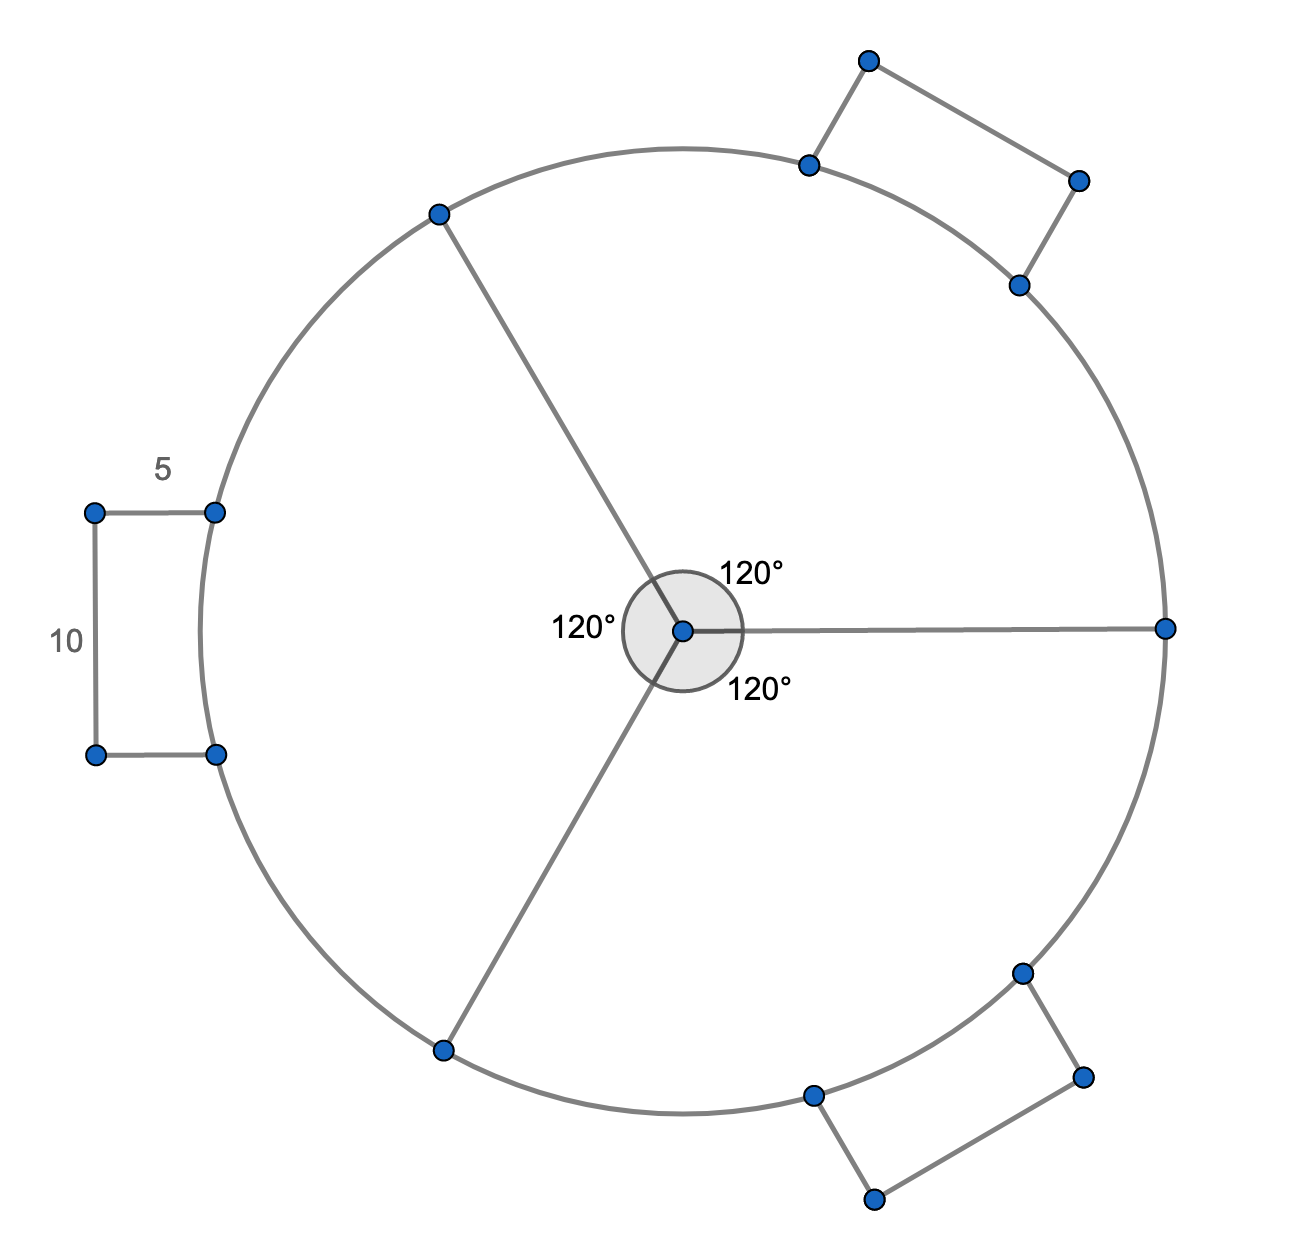
\includegraphics[scale=0.15]{ground.png}
    \caption{比赛场地俯视图}
    \end{figure}
\end{itemize}

\begin{itemize}
\item
  巧取智夺:蛋碰撞箱为一个直径 \(0.7\text{ m}\)
  的圆形。角色成功抱起蛋的条件是:

  \begin{enumerate}
  \def\labelenumi{\arabic{enumi}.}
  \item
    蛋在地上且角色外边缘和蛋表面距离不超过
    \(0.1\text{ m}\)(即,角色与蛋的圆心距小于半径之和加此距离);如果多个角色满足此条件,且在同一个时刻尝试抱起,则距离蛋最近的成功抱起;
  \item
    蛋在另一个角色身上(无论敌我);那么,抱起蛋的角色会把蛋举在头上,即蛋碰撞箱中心和角色碰撞箱中心重合;距离要求与上条相同;如果有多个人尝试抢,则最近的成功抢过来;
  \end{enumerate}
\item
  精准入篮:放下蛋时,可以在所有保证蛋和糖豆人相切的位置放置;但是蛋不能卡在别人身上,也不能和其他蛋重叠或卡入地图边界;蛋在外围
  \(3\) 个区域内时判断为入篮,具体判断点为蛋的中心。
\end{itemize}

\hypertarget{header-n26}{%
\section{参赛流程}\label{header-n26}}

\hypertarget{header-n27}{%
\subsection{加入小组}\label{header-n27}}

请在小组页面加入本次比赛的小组。

\hypertarget{header-n29}{%
\subsection{下载游戏包}\label{header-n29}}

在右上角的「下载游戏包」按钮下载游戏包。游戏包内含:

\begin{itemize}
\item
  开发\texttt{SDK}与简单的样例AI;
\item
  本地评测程序;
\item
  开发说明。
\end{itemize}

\hypertarget{header-n39}{%
\subsection{编写 AI}\label{header-n39}}

请参考游戏包中的开发说明与样例,选择你喜欢的语言编写
AI。详细的配置说明在开发说明中都有提及。

\hypertarget{header-n41}{%
\subsection{提交代码}\label{header-n41}}

在「我的AI」处提交自己的
AI,可根据实际情况选择对应编译语言,编译成功后便可将 AI 派遣到对应比赛。

\hypertarget{header-n43}{%
\subsection{派遣 AI}\label{header-n43}}

您可以在天梯上派遣AI,并发起对战,以观测己方与其他选手的策略博弈。天梯成绩仅供参考,不计入最终比赛名次成绩。

\hypertarget{header-n45}{%
\subsection{观看回放}\label{header-n45}}

您可以在 \url{https://egg-display.netlify.app/} 上传回放文件,观看比赛回放。\\
您也可以使用 Saiblo 在对局结束后打开的窗口中的播放器。

\hypertarget{header-n47}{%
\subsection{决出名次}\label{header-n47}}

初赛时间截止后,我们会在提交了代码的选手间发起大量对局并统计积分,直至排名收敛为止。

\hypertarget{header-n49}{%
\subsection{测试方法}\label{header-n49}}

\hypertarget{header-n50}{%
\subsubsection{本地测试}\label{header-n50}}

我们提供了一个本地裁判程序(下面假设你把它放在\texttt{./judger.py})
用于评测两个本地 AI,具体使用方法为:

\begin{enumerate}

\item 下载裁判程序、游戏逻辑(假设命名为\texttt{eggs}),放在SDK根目录。
\item 我们假设你采用Python SDK,且当前命令行在 \texttt{main.py} 所在目录。执行下列命令,进入调试模式:

\begin{lstlisting}[language=bash]
$ python ./judger.py test_mode
\end{lstlisting}
进入调试模式后界面如下:
\begin{lstlisting}
You can input help to know the instrution set
> 
\end{lstlisting}

\item 在调试模式依次逐行输入下列语句,以使用\texttt{main.py}中的AI分别控制3个队伍,运行一次测试:
\begin{lstlisting}
0 0 python+main.py
0 1 python+main.py
0 2 python+main.py
4 eggs dummyConfig replay.bin
\end{lstlisting}
\end{enumerate}

对局完成后,会将对局文件存入 \texttt{replay.bin} 。

注意:请确保本地执行 \texttt{python} 命令呼出的是 \textsc{Python 3}.

\hypertarget{header-n58}{%
\subsubsection{评测逻辑文件下载}\label{header-n58}}

出于安全考虑,评测逻辑只提供构建好的版本。\par 请在
\url{https://github.com/ssast-tech/thuai-egg-releases}
进行下载,或者直接采用「下载游戏包」页面的链接。

请注意:考虑到选手电脑的性能问题,我们在用于本地评测的逻辑中放宽了时间限制;实际在Saiblo评测时,单次\texttt{update}的时间限制是 \SI{0.1}{\second}. 
如果任何一个回合超出这个限制,对应的AI\color{red}此回合的回复会被抛弃\color{black},但是你的AI\color{red}仍然可以参与后续回合的交互\color{black}。

关于 AI 调试:如果你想要看到更多来自游戏逻辑的调试信息,只需要重命名逻辑文件名使得其包含 \texttt{verbose} 这一字符串即可。
你可能需要对上述调试模式输入语句的最后一行做适当更改,以匹配重命名后的逻辑文件名。
\end{document}
